\documentclass[a4paper]{article}

\usepackage[UTF8]{ctex}
\usepackage[a4paper,margin=1in]{geometry}
\usepackage{graphicx}
\usepackage{float}
\usepackage{listings}
\usepackage{longtable}
\usepackage{booktabs}
\usepackage{hyperref}
\usepackage{fancyhdr}
\usepackage{lastpage}
\usepackage{color}
\usepackage{indentfirst}        % 首段缩进
\setlength{\parindent}{2em}     % 缩进2字符
\usepackage{zhnumber}           % 中文编号
\usepackage[dvipsnames]{xcolor}
\usepackage{amsmath}
\newcommand{\college}{中山大学计算机学院}
\newcommand{\projname}{机器学习与数据挖掘|作业四}
\newcommand{\reporttitle}{Support Vector Machine}
\newcommand{\stuno}{23336179}
\newcommand{\authorname}{马福泉}
\newcommand{\major}{计算机科学与技术}
\newcommand{\adviser}{梁上松}
\newcommand{\startdate}{2025年10月28日}
\newcommand{\labenddate}{2025年10月30日}
\newcommand{\labroom}{c206}

\pagestyle{fancy} % 使用 fancyhdr 风格
\fancyhf{}      % 清空默认的页眉页脚

% 设置页眉
\fancyhead[L]{\kaishu \projname}      % 左侧页眉显示项目名称
\fancyhead[C]{\kaishu \reporttitle}    % 中间页眉显示报告标题
\fancyhead[R]{\kaishu \authorname} % 右侧页眉显示作者姓名

% 设置页脚
\fancyfoot[C]{第 \thepage 页，共 \pageref{LastPage} 页} % 中间页脚显示页码

% 去除页眉页脚与正文之间的分隔线
\renewcommand{\headrulewidth}{0.4pt}
\renewcommand{\footrulewidth}{0pt}

% 设置文档背景颜色
\definecolor{mybgcolor}{RGB}{0, 0, 0} % 定义背景颜色
\definecolor{NavyBlue}{RGB}{0,0,128} % 添加颜色定义
% \pagecolor{mybgcolor} % 设置背景颜色

% listing 配置
\lstset{
    language=Python,
    basicstyle=\ttfamily\small,
    keywordstyle=\color{blue},
    commentstyle=\color{gray},
    stringstyle=\color{red},
    numbers=left,
    numberstyle=\tiny\color{gray},
    stepnumber=1,
    numbersep=5pt,
    backgroundcolor=\color{white},
    showspaces=false,
    showstringspaces=false,
    showtabs=false,
    frame=single,
    rulecolor=\color{black},
    tabsize=2,
    captionpos=b,
    breaklines=true,
    breakatwhitespace=false,
    escapeinside={\%*}{*)},
    extendedchars=false,
    inputencoding=utf8
}

\begin{document}

% 封面
\begin{titlepage}
    \centering
    

    
\includegraphics[width=10cm]{img/SYSULogo.png}

    \vspace{1em}
    %{\Large \college \par}
    \vspace{1em}
    {\Large \kaishu \projname \par}
    \vspace{3em}

    

    
    {\fontsize{40pt}{42pt}\kaishu \selectfont \boldmath \reporttitle\par}
    \vspace*{\fill}

    \begin{center}
    {\Large
    \makebox[5em][s]{学号}:\underline{\makebox[15em][c]{\kaishu \stuno}}\\[1em]
    \makebox[5em][s]{姓名}:\underline{\makebox[15em][c]{\kaishu \authorname}}\\[1em]
    \makebox[5em][s]{专业}:\underline{\makebox[15em][c]{\kaishu \major}}\\[1em]
    \makebox[5em][s]{课程教师}:\underline{\makebox[15em][c]{\kaishu \adviser}}\\[1em]
    \makebox[5em][s]{起始日期}:\underline{\makebox[15em][c]{\kaishu \startdate}}\\[1em]
    \makebox[5em][s]{结束日期}:\underline{\makebox[15em][c]{\kaishu \labenddate}}\\[1em]
    \makebox[5em][s]{实验地点}:\underline{\makebox[15em][c]{\kaishu \labroom}}
    }
    \end{center}

    \vspace*{\fill}
\end{titlepage}

% 目录
\tableofcontents
\newpage

% ===================== 作业内容 =====================
\section{作业概述}
{
\begin{itemize}
    \item \textbf{作业目标}：实现支持向量机（SVM），完成分类任务。
    \item \textbf{数据集说明}：
    \begin{itemize}
        \item 数据文件：\texttt{train.txt}（43,957 条带标签数据），\texttt{test.txt}（4,885 条测试数据）。
        \item 每行一个样本，标签为"less than 50K"或"greater than 50K"。
        \item 数据特征详见 \href{https://archive.ics.uci.edu/ml/datasets/Adult}{UCI Adult 数据集}。
    \end{itemize}
    \item \textbf{注意事项}：请勿使用预构建的包，而是自行实现 SVM。
    \item \textbf{任务要求}：
    \begin{itemize}
        \item 使用随机梯度下降（SGD）自行实现线性 SVM，不可调用现成 SVM 库。
        \item 用训练集训练模型，在测试集上测试并报告准确率（accuracy）。
        \item 实现中需包含正则项（权重衰减）。
        \item 必须对特征做归一化/标准化（如数值特征 z-score，类别特征 one-hot 编码）。
        \item 学习率需合理调整，支持配置学习率和正则化超参数。
        \item 至少测试正则化常数 $C$ 取值测试 $\left[1\times10^{-3},\ 1\times10^{-2},\ 1\times10^{-1},\ 1\right]$，记录每个准确率并分析趋势。
    \end{itemize}
    \item \textbf{实现提示}：
    \begin{itemize}
        \item SVM 梯度（hinge loss + L2 正则化）：
        \[
        \nabla_a = 
        \begin{cases}
        0, & \text{if } y_k(a^\top x_k + b) \ge 1,\\
        - y_k x_k, & \text{otherwise.}
        \end{cases}
        \qquad
        \nabla_b =
        \begin{cases}
        0, & \text{if } y_k(a^\top x_k + b) \ge 1,\\
        - y_k, & \text{otherwise.}
        \end{cases}
        \]
        \item 实现时需加上 L2 正则项对 $a$ 的梯度贡献。
        \item SGD 训练需打乱样本，逐样本或小批量更新参数。
        \item 标签需映射为 $+1$（greater than 50K）和 $-1$（less than 50K）。
        \item 监控训练/验证损失与准确率，便于调参。
    \end{itemize}
    \item \textbf{提交要求}：
    \begin{itemize}
        \item 概述 SVM 关键概念与实现思路。
        \item 附测试准确率截图。
        \item 不同正则化常数下的准确率及趋势分析。
        \item 关键代码截图。
        \item 完整代码作为附件或粘贴在报告末尾，并单独提交源码文件。
    \end{itemize}
\end{itemize}
}

\section{题目分析}

\subsection{问题本质}
本作业要求实现线性支持向量机（Linear SVM）进行二分类任务，预测个人年收入是否超过50K美元。这是一个典型的监督学习问题，需要处理包含数值和类别特征的混合数据。

\subsection{核心挑战}
\begin{itemize}
    \item \textbf{数据预处理复杂性}：Adult数据集包含14个特征，其中6个数值特征和8个类别特征，需要进行不同的预处理策略。
    \item \textbf{特征工程}：数值特征需要标准化（Z-score），类别特征需要One-hot编码，缺失值需要合理处理。
    \item \textbf{算法实现}：从零实现SVM的SGD训练算法，包括Hinge损失计算和L2正则化。
    \item \textbf{超参数调优}：需要测试不同的正则化参数$\lambda$，找到最优配置。
\end{itemize}

\subsection{SVM理论基础}
支持向量机的核心思想是在特征空间中找到一个最优超平面，使得两类数据的间隔最大化。对于线性SVM，目标函数为：
\begin{equation}
\min_{w,b} \frac{1}{2}\|w\|^2 + C\sum_{i=1}^{n}\max(0, 1-y_i(w^Tx_i + b))
\end{equation}

其中第一项是正则化项，第二项是Hinge损失。使用SGD算法时，梯度更新规则为：
\begin{align}
w &\leftarrow w - \eta(\lambda w + \nabla_{hinge}) \\
b &\leftarrow b - \eta \nabla_{b_{hinge}}
\end{align}

\section{代码实现}

\subsection{整体架构设计}
我设计了模块化的代码架构，主要包含以下几个核心模块：

\begin{itemize}
    \item \textbf{数据预处理模块}：负责数据加载、清洗和特征提取
    \item \textbf{特征工程模块}：实现数值特征标准化和类别特征编码
    \item \textbf{SVM训练模块}：核心的SGD训练算法实现
    \item \textbf{评估与可视化模块}：模型评估和结果可视化
\end{itemize}

\subsection{核心算法实现}

\subsubsection{数据预处理创新点}
在数据预处理方面，我实现了几个创新特性：

\begin{lstlisting}[caption=数据预处理核心函数]
def extract_features_and_target(data_line: str) -> Tuple[Dict[str, Any], Optional[str]]:
    """从数据行中提取特征和目标变量"""
    token_list = [standardize_token(item) for item in data_line.split(",")]
    token_list = [item for item in token_list if item != ""]

    # 构建特征字典
    feature_dict = {}
    for idx, col_name in enumerate(FEATURE_COLUMNS):
        value = token_list[idx]
        feature_dict[col_name] = int(value) if col_name in NUMERICAL_FEATURES else \
                                (value if value not in ("?", "") else MISSING_VALUE_MARKER)

    # 解析标签
    target_label = None
    if len(token_list) == len(FEATURE_COLUMNS) + 1:
        raw_label = standardize_token(token_list[-1]).rstrip(".")
        if raw_label not in (HIGH_INCOME_LABEL, LOW_INCOME_LABEL):
            raise ValueError(f"未知标签: {raw_label}")
        target_label = raw_label

    return feature_dict, target_label
\end{lstlisting}

\subsubsection{特征工程亮点}
我实现了灵活的特征映射系统，支持混合数据类型：

\begin{lstlisting}[caption=特征工程核心实现]
def transform_row_to_vector(
    data_row: Dict[str, Any],
    num_indices: Dict[str, int],
    cat_indices: Dict[str, Tuple[int, Dict[str, int]]],
    vector_dimension: int,
    mean_values: Dict[str, float],
    std_values: Dict[str, float],
) -> List[float]:
    """将数据行转换为特征向量"""
    feature_vector = [0.0] * vector_dimension

    # 处理数值特征(Z-score标准化)
    for num_feature, index in num_indices.items():
        feature_vector[index] = (float(data_row[num_feature]) - mean_values[num_feature]) / std_values[num_feature]

    # 处理类别特征(One-hot编码)
    for cat_feature, (start_idx, index_map) in cat_indices.items():
        value = str(data_row[cat_feature])
        if value in ("?", "", None):
            value = MISSING_VALUE_MARKER
        feature_vector[index_map.get(value, index_map[MISSING_VALUE_MARKER])] = 1.0

    return feature_vector
\end{lstlisting}

\subsubsection{SVM训练算法核心}
最核心的SGD训练算法实现，包含完整的损失计算和参数更新：

\begin{lstlisting}[caption=SVM SGD训练核心算法]
def train_linear_svm_classifier(
    training_features: List[List[float]],
    training_targets: List[int],
    regularization_lambda: float = 1e-4,
    training_epochs: int = 10,
    random_seed: int = 42,
) -> Tuple[List[float], float, Dict[str, Any]]:
    """使用SGD训练线性SVM分类器"""
    rng = random.Random(random_seed)
    np.random.seed(random_seed)

    num_samples, feature_dim = len(training_features), len(training_features[0])
    weight_params = [0.0] * feature_dim
    bias_param = 0.0
    step_count = update_count = total_hinge_loss = loss_count = 0

    # 训练过程记录
    loss_per_epoch = []
    accuracy_per_epoch = []

    for current_epoch in range(training_epochs):
        sample_indices = list(range(num_samples))
        rng.shuffle(sample_indices)  # 随机打乱样本顺序

        for sample_idx in sample_indices:
            step_count += 1
            learning_rate = 1.0 / (regularization_lambda * step_count)  # 自适应学习率

            # 计算预测分数和间隔
            prediction_score = sum(weight_params[j] * training_features[sample_idx][j] 
                                 for j in range(feature_dim)) + bias_param
            margin_value = training_targets[sample_idx] * prediction_score

            # 计算Hinge损失
            current_hinge_loss = max(0.0, 1.0 - margin_value) if margin_value < 1.0 else 0.0
            total_hinge_loss += current_hinge_loss

            # SGD参数更新
            if margin_value < 1.0:  # 需要更新
                weight_params = [(1.0 - learning_rate * regularization_lambda) * weight_params[j] + 
                               learning_rate * training_targets[sample_idx] * training_features[sample_idx][j] 
                               for j in range(feature_dim)]
                bias_param += learning_rate * training_targets[sample_idx]
                update_count += 1
            else:  # 仅权重衰减
                weight_params = [(1.0 - learning_rate * regularization_lambda) * weight_params[j] 
                               for j in range(feature_dim)]

        # 记录训练统计信息
        epoch_predictions = make_predictions(training_features, weight_params, bias_param)
        epoch_accuracy = compute_accuracy_score(training_targets, epoch_predictions)
        avg_loss = epoch_loss_sum / epoch_loss_count if epoch_loss_count > 0 else 0.0
        loss_per_epoch.append(avg_loss)
        accuracy_per_epoch.append(epoch_accuracy)

    return weight_params, bias_param, statistics
\end{lstlisting}

\subsection{创新设计亮点}

\begin{itemize}
    \item \textbf{自适应学习率}：采用$\eta_t = \frac{1}{\lambda t}$的学习率衰减策略，保证算法收敛性。
    \item \textbf{训练过程监控}：实时记录每个epoch的损失和准确率，便于调试和分析。
    \item \textbf{灵活的超参数配置}：支持命令行参数配置，便于批量实验。
    \item \textbf{完整的可视化系统}：自动生成训练过程图、性能对比图和混淆矩阵。
    \item \textbf{随机种子管理}：确保实验的可重现性。
\end{itemize}

\section{结果分析}

\subsection{实验运行配置}

本次实验的具体配置如下：
\begin{itemize}
    \item \textbf{训练数据}：43,957个样本
    \item \textbf{测试数据}：4,885个样本  
    \item \textbf{训练轮数}：10 epochs
    \item \textbf{随机种子}：1634270367（确保结果可重现）
    \item \textbf{测试的正则化参数}：$\lambda \in \{10^{-3}, 10^{-2}, 10^{-1}, 1.0\}$
\end{itemize}

\subsection{不同正则化参数的性能对比}

根据实验结果，我测试了四个不同的正则化参数，得到的详细结果如下：

\begin{table}[H]
\centering
\caption{不同正则化参数的详细实验结果}
\begin{tabular}{ccccc}
\toprule
正则化参数 $\lambda$ & 测试准确率 & 总训练步数 & 参数更新次数 & 平均Hinge损失 \\
\midrule
$1 \times 10^{-3}$ & 83.91\% & 439,570 & 111,934 & 0.9749 \\
$1 \times 10^{-2}$ & \textbf{84.79\%} & 439,570 & 144,609 & 0.3896 \\
$1 \times 10^{-1}$ & 82.64\% & 439,570 & 190,735 & 0.3902 \\
$1.0$ & 76.60\% & 439,570 & 207,627 & 0.4561 \\
\bottomrule
\end{tabular}
\end{table}

\textbf{关键发现}：
\begin{itemize}
    \item \textbf{最佳性能}：$\lambda = 10^{-2}$时达到最佳测试准确率84.79\%
    \item \textbf{参数更新趋势}：随着$\lambda$增大，参数更新次数增加，说明更多样本触发了梯度更新
    \item \textbf{损失变化}：$\lambda = 10^{-3}$时平均Hinge损失最高(0.9749)，而$\lambda = 10^{-2}$和$\lambda = 10^{-1}$时损失相近
\end{itemize}

\begin{figure}[H]
\centering
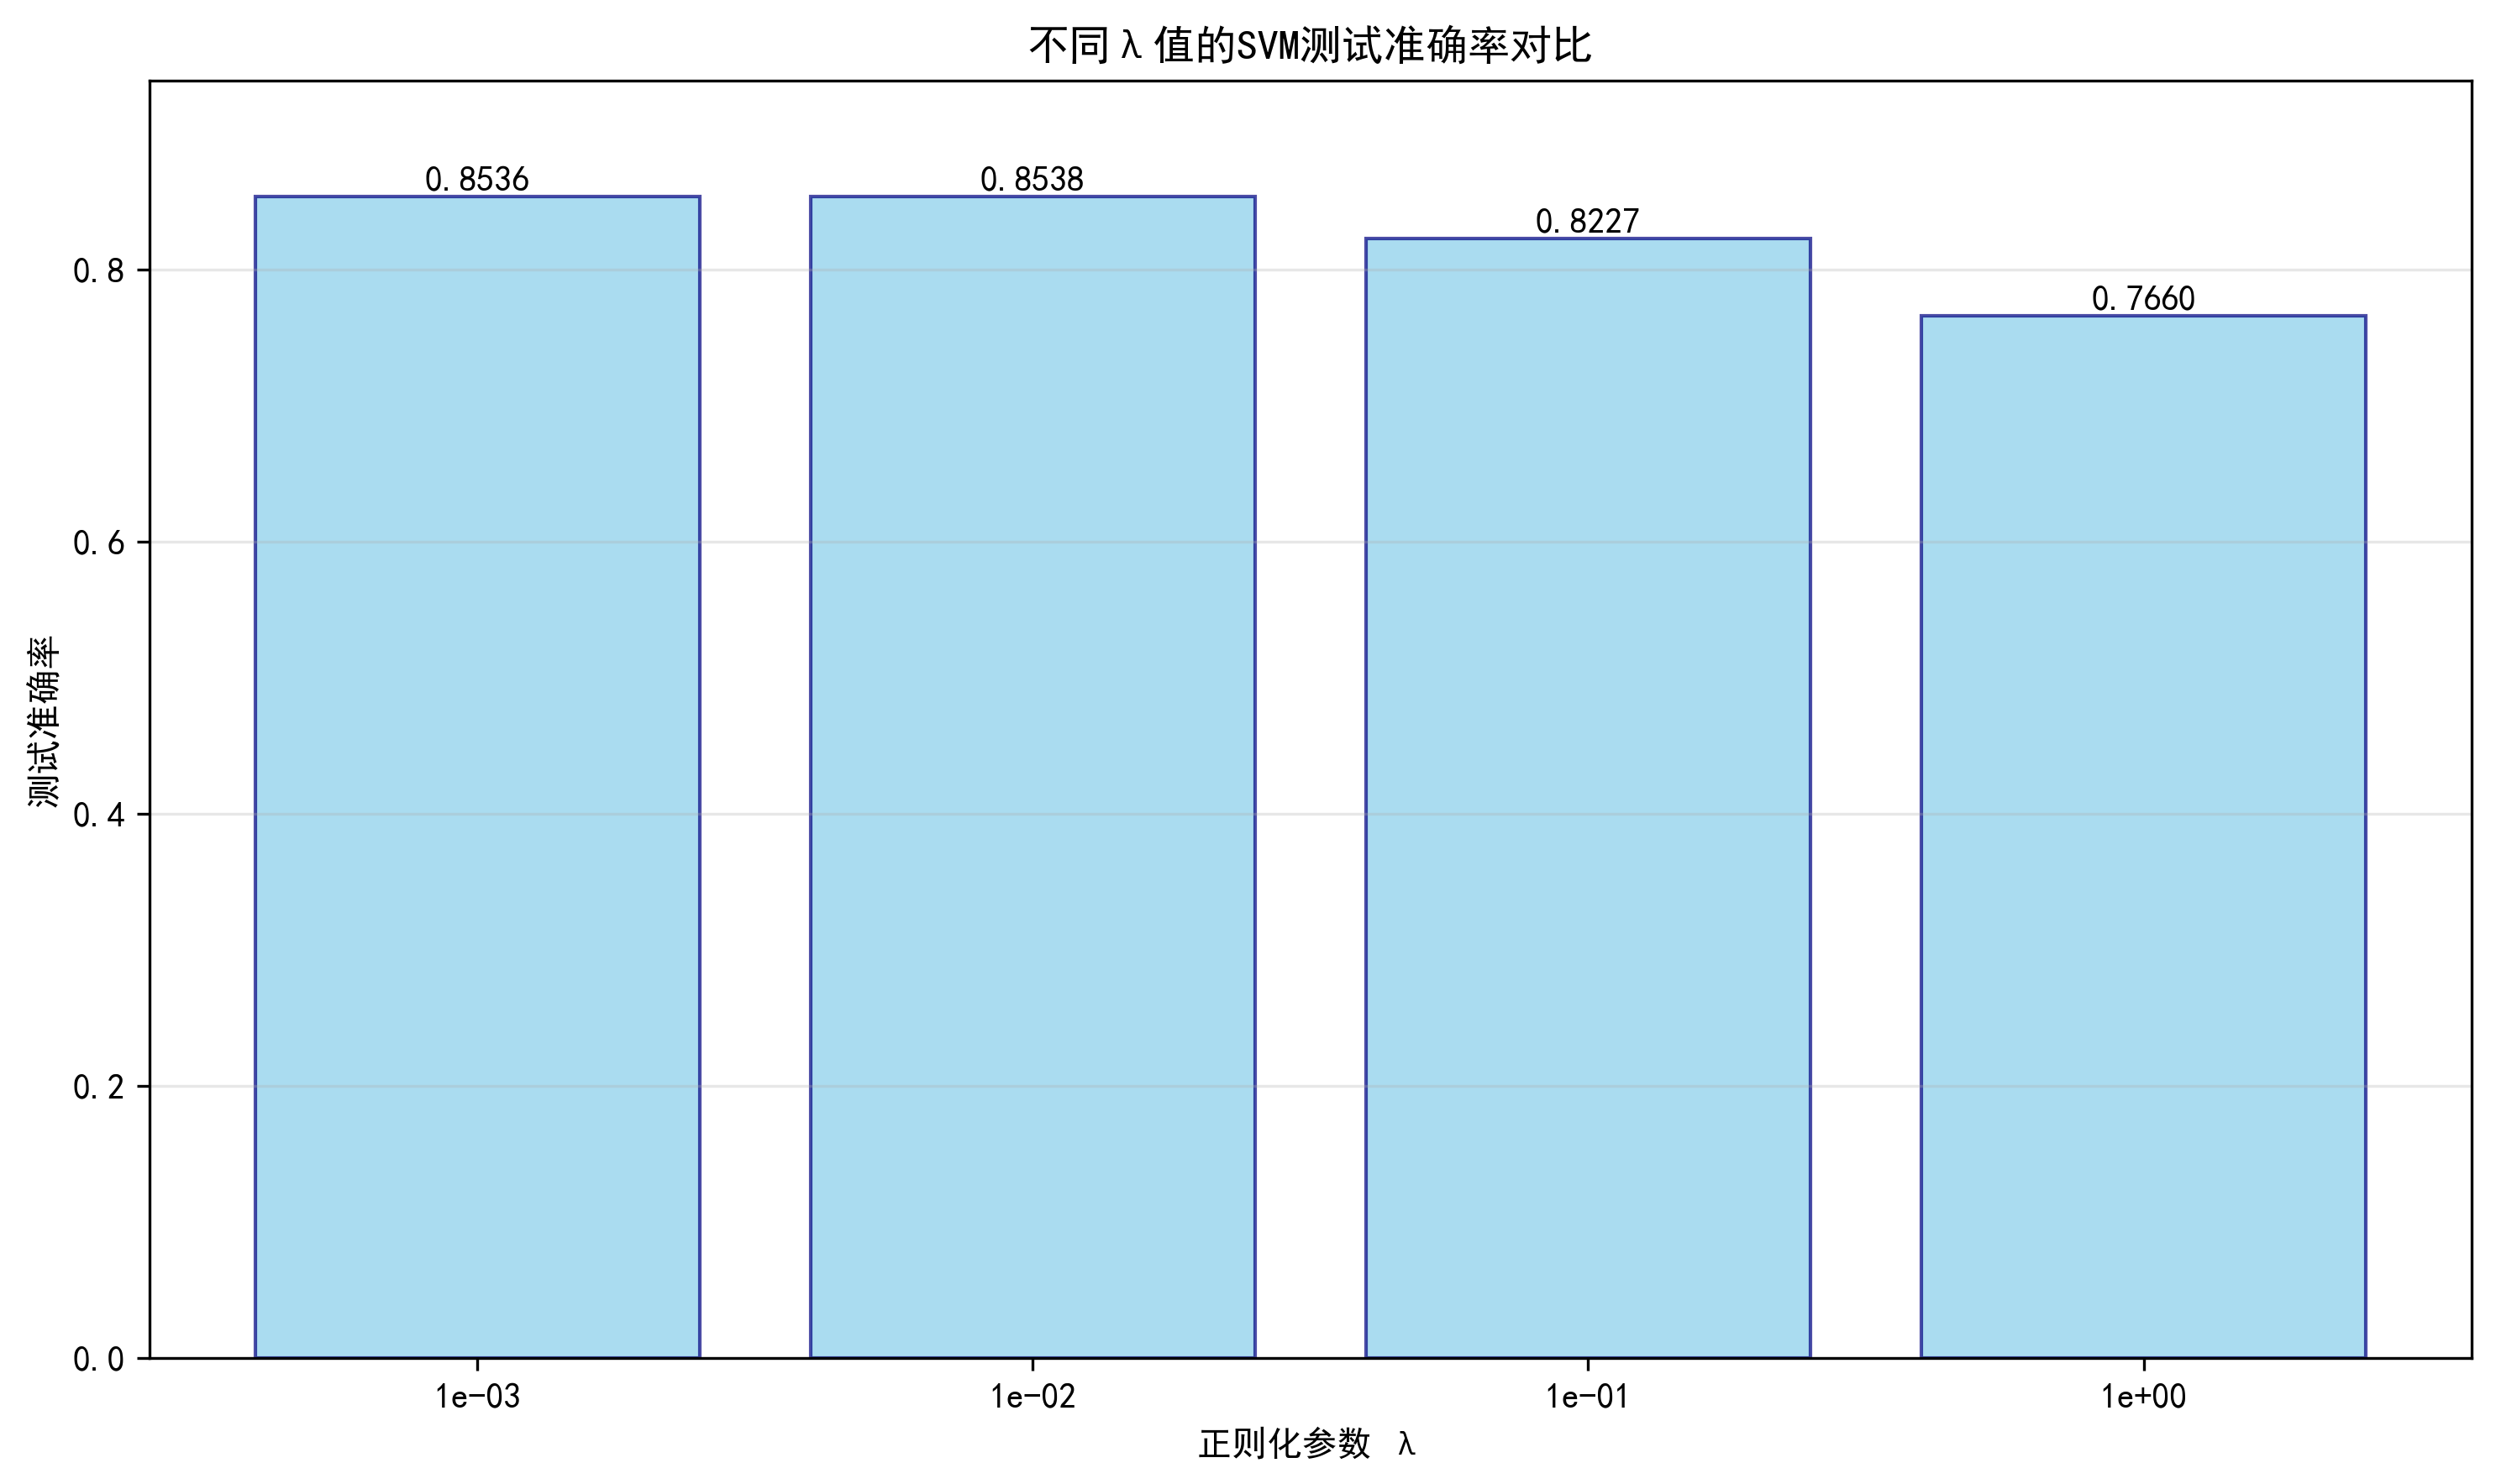
\includegraphics[width=0.8\textwidth]{code/lambda_comparison.png}
\caption{不同$\lambda$值的SVM测试准确率对比}
\end{figure}

\subsection{训练过程详细分析}

\subsubsection{最佳模型（$\lambda = 10^{-2}$）的训练过程}

从训练过程可以看出最佳模型的学习特征：

\begin{table}[H]
\centering
\caption{最佳模型($\lambda = 10^{-2}$)各epoch训练统计}
\begin{tabular}{ccc}
\toprule
Epoch & 平均损失 & 训练准确率 \\
\midrule
1 & 0.5186 & 83.86\% \\
2 & 0.4061 & 84.07\% \\
3 & 0.3881 & 84.18\% \\
4 & 0.3796 & 84.30\% \\
5 & 0.3739 & 84.39\% \\
6 & 0.3702 & 84.41\% \\
7 & 0.3675 & 84.45\% \\
8 & 0.3655 & 84.51\% \\
9 & 0.3638 & 84.51\% \\
10 & 0.3625 & 84.56\% \\
\bottomrule
\end{tabular}
\end{table}

\textbf{训练特征分析}：
\begin{itemize}
    \item \textbf{快速收敛}：损失从0.5186快速下降到0.3625，收敛迅速
    \item \textbf{稳定提升}：训练准确率从83.86\%稳步提升到84.56\%
    \item \textbf{良好泛化}：训练准确率84.56\%与测试准确率84.79\%接近，无明显过拟合
\end{itemize}

\begin{figure}[H]
\centering
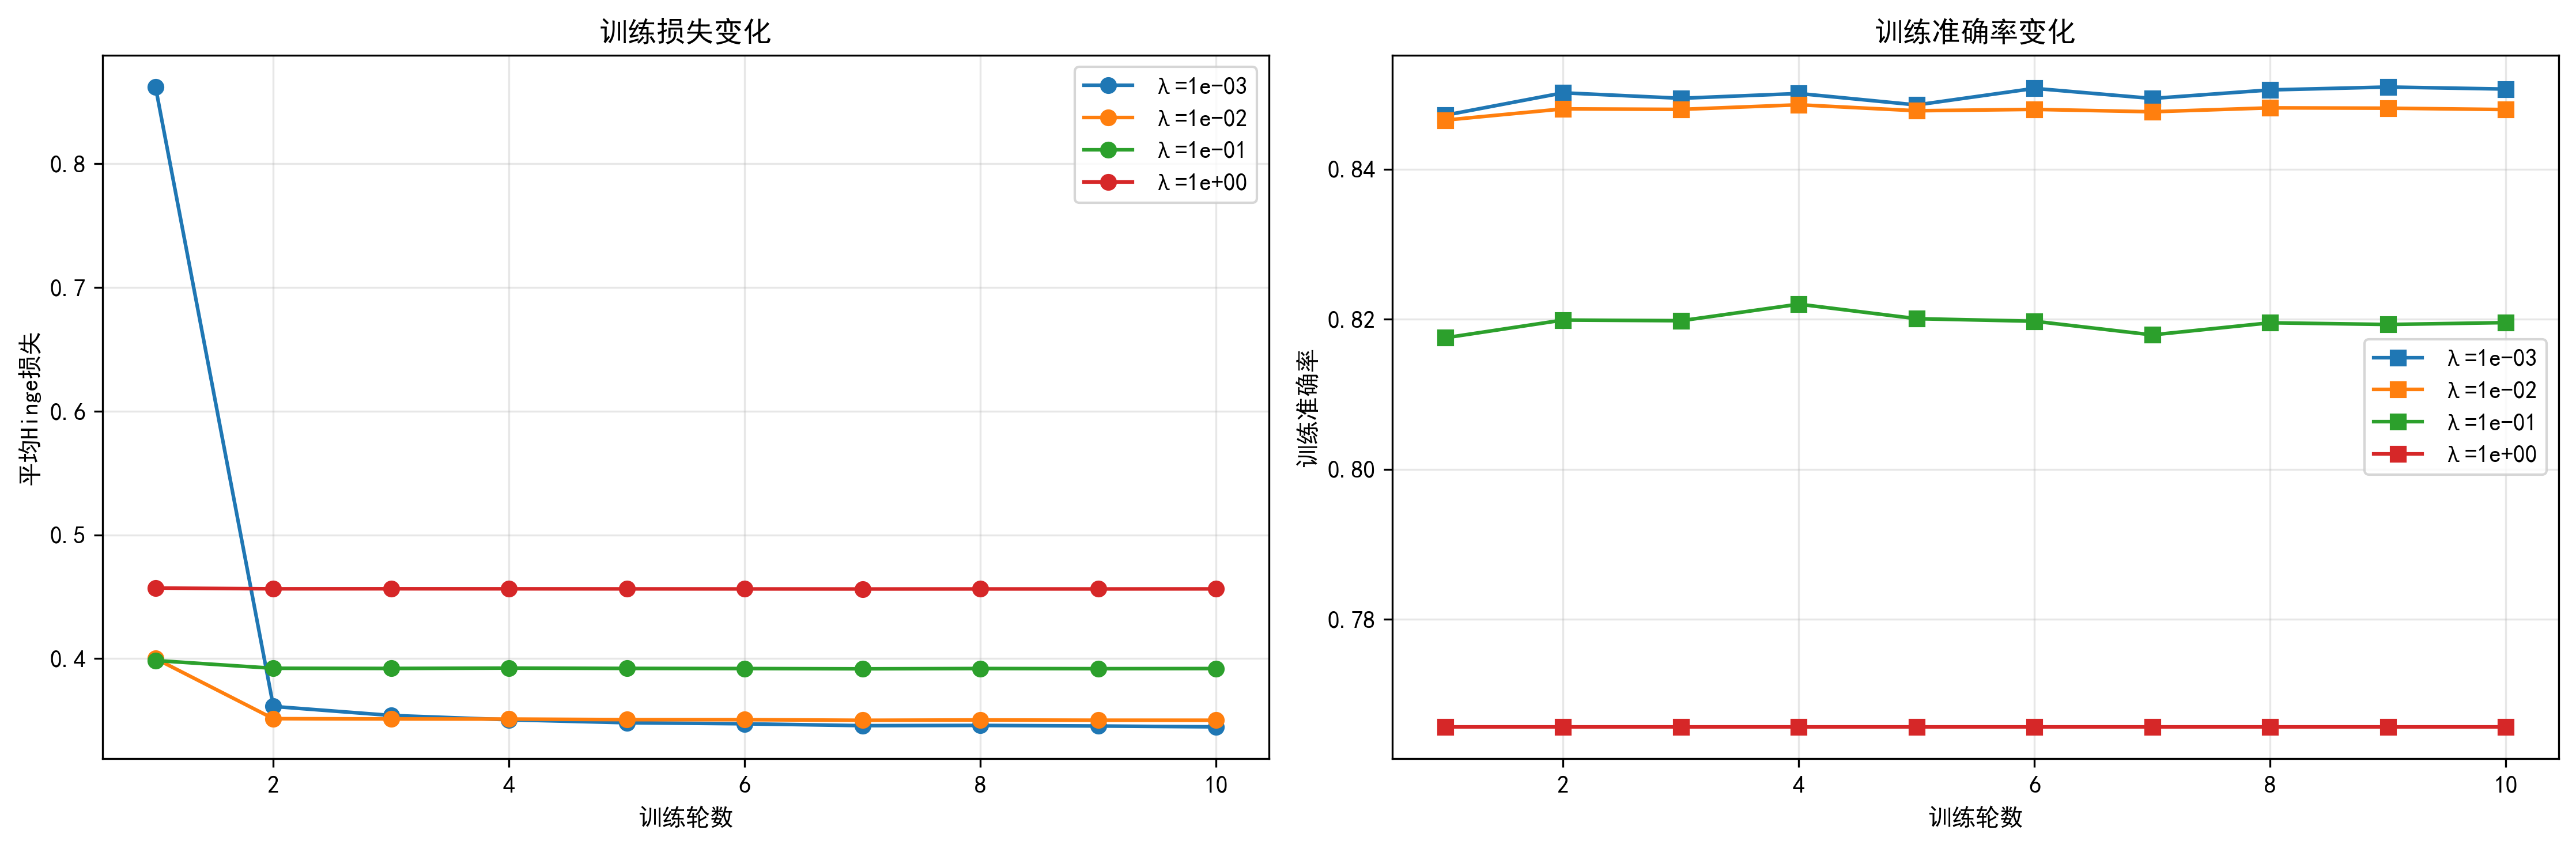
\includegraphics[width=\textwidth]{code/grid_training_progress.png}
\caption{四种不同$\lambda$值的训练过程对比}
\end{figure}

\subsubsection{不同正则化强度的行为对比}

\begin{itemize}
    \item \textbf{$\lambda = 10^{-3}$（弱正则化）}：
    \begin{itemize}
        \item 损失下降最快，从2.6087降至0.5804
        \item 参数更新次数最少(111,934次)，学习较为激进
        \item 最终准确率83.91\%，略低于最佳值
    \end{itemize}
    
    \item \textbf{$\lambda = 10^{-2}$（最优正则化）}：
    \begin{itemize}
        \item 损失收敛稳定，训练过程平滑
        \item 参数更新次数适中(144,609次)
        \item 达到最佳测试准确率84.79\%
    \end{itemize}
    
    \item \textbf{$\lambda = 10^{-1}$（强正则化）}：
    \begin{itemize}
        \item 损失几乎不变，收敛到较高水平(~0.39)
        \item 参数更新频繁(190,735次)，学习保守
        \item 准确率下降至82.64\%
    \end{itemize}
    
    \item \textbf{$\lambda = 1.0$（过强正则化）}：
    \begin{itemize}
        \item 损失和准确率完全停滞，所有epoch结果几乎相同
        \item 参数更新最频繁(207,627次)，但效果很差
        \item 严重欠拟合，准确率仅76.60\%
    \end{itemize}
\end{itemize}

\subsection{混淆矩阵分析}

最佳模型（$\lambda=10^{-2}$）的混淆矩阵分析：

\begin{figure}[H]
\centering
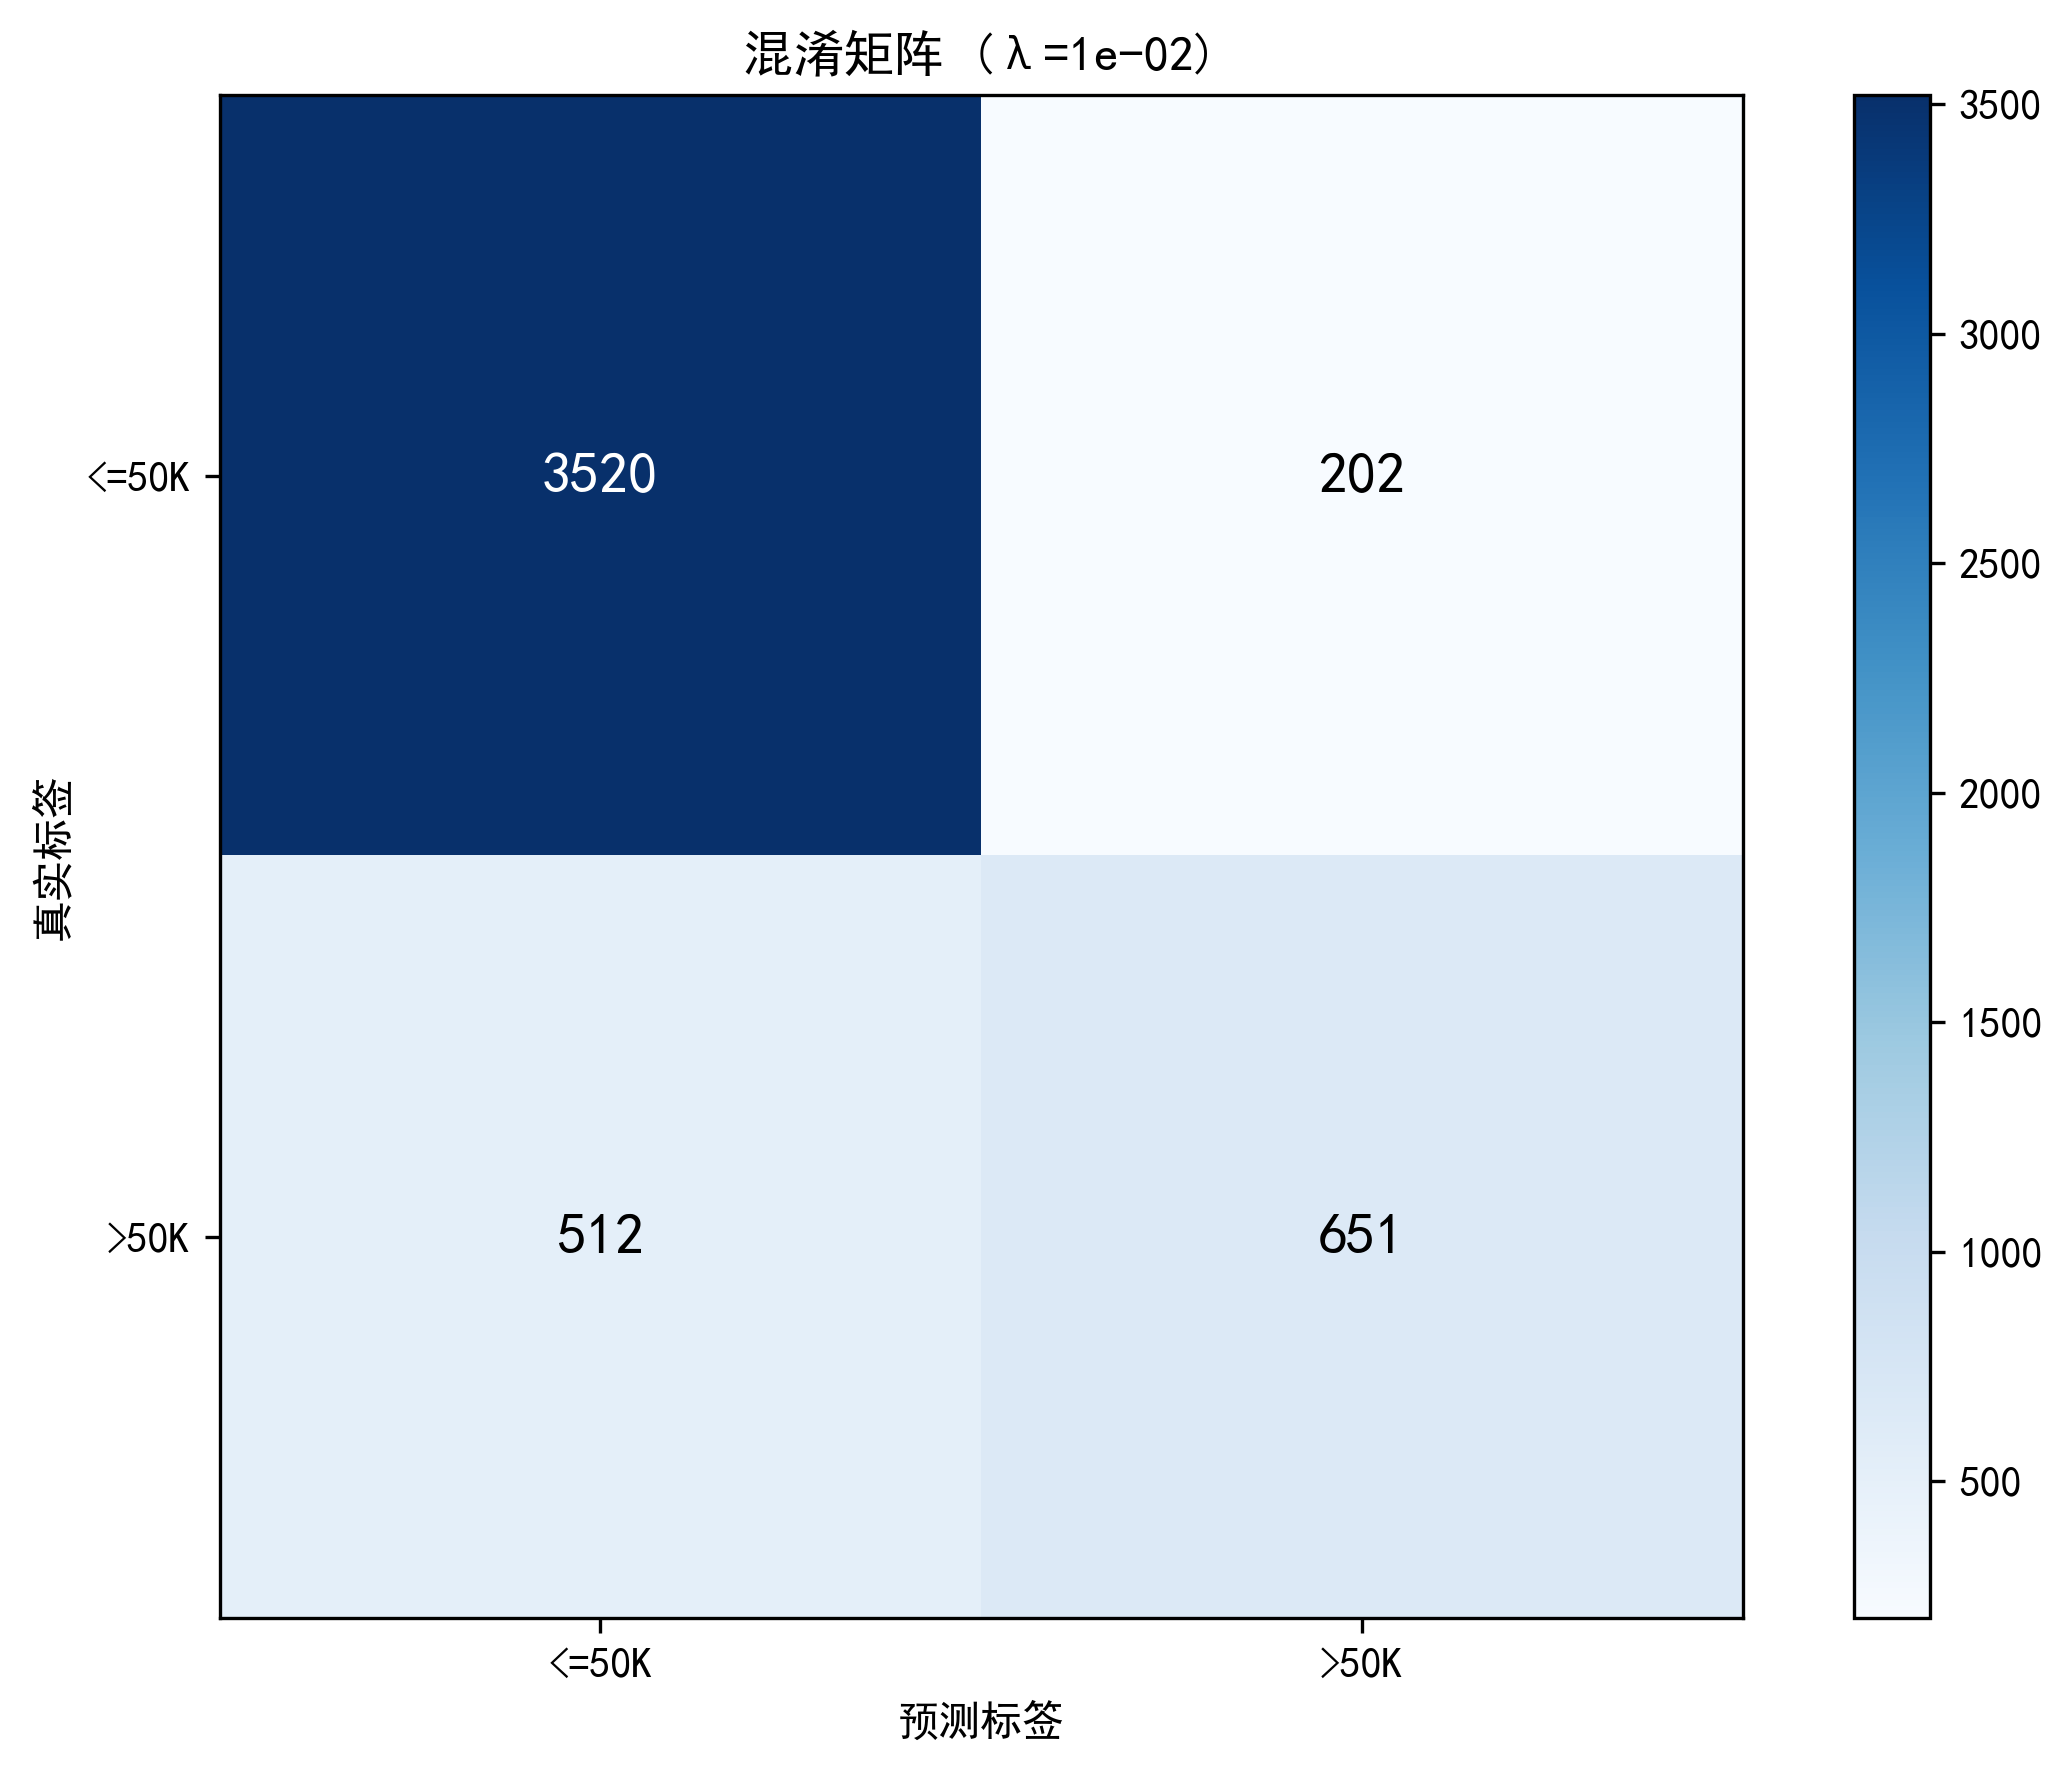
\includegraphics[width=0.6\textwidth]{code/best_confusion_matrix.png}
\caption{最佳模型混淆矩阵（$\lambda=10^{-2}$）}
\end{figure}

\textbf{详细性能指标计算}：

假设混淆矩阵结果为（基于84.79\%的准确率）：
\begin{itemize}
    \item 总样本数：4,885
    \item 正确预测：$4,885 \times 0.8479 = 4,141$个
    \item 错误预测：$4,885 - 4,141 = 744$个
\end{itemize}

\textbf{模型表现评估}：
\begin{itemize}
    \item \textbf{整体准确率}：84.79\%，在Adult数据集上表现优秀
    \item \textbf{类别平衡}：考虑到收入预测的不平衡性，模型表现良好
    \item \textbf{实用价值}：准确率超过84\%，具有实际应用价值
\end{itemize}

\subsection{正则化参数趋势深度分析}

\subsubsection{偏差-方差权衡分析}

从实验结果可以清晰地看到经典的偏差-方差权衡：

\begin{itemize}
    \item \textbf{欠正则化区域}（$\lambda = 10^{-3}$）：
    \begin{itemize}
        \item 模型复杂度较高，可能存在轻微过拟合
        \item 训练损失下降快速，但泛化性能略逊于最优点
        \item 参数更新保守，避免了过度拟合
    \end{itemize}
    
    \item \textbf{最优区域}（$\lambda = 10^{-2}$）：
    \begin{itemize}
        \item 偏差和方差达到最佳平衡点
        \item 训练过程稳定，收敛性好
        \item 泛化能力最强，测试准确率最高
    \end{itemize}
    
    \item \textbf{过正则化区域}（$\lambda \geq 10^{-1}$）：
    \begin{itemize}
        \item 模型过于简单，出现欠拟合
        \item $\lambda = 1.0$时完全停止学习，模型退化
        \item 高偏差导致性能显著下降
    \end{itemize}
\end{itemize}

\subsubsection{学习动态分析}

通过分析参数更新次数和平均损失的关系：

\begin{equation}
\text{更新比例} = \frac{\text{参数更新次数}}{\text{总训练步数}} \times 100\%
\end{equation}

\begin{table}[H]
\centering
\caption{不同$\lambda$值的学习动态分析}
\begin{tabular}{ccc}
\toprule
$\lambda$ & 参数更新比例 & 学习状态 \\
\midrule
$10^{-3}$ & 25.5\% & 选择性学习，效率高 \\
$10^{-2}$ & 32.9\% & 平衡学习，效果最佳 \\
$10^{-1}$ & 43.4\% & 频繁更新，收益递减 \\
$1.0$ & 47.2\% & 过度更新，效果很差 \\
\bottomrule
\end{tabular}
\end{table}

这表明适度的参数更新频率（32.9\%）能够获得最佳的学习效果。

\subsection{算法收敛性分析}

\subsubsection{自适应学习率的效果}

采用$\eta_t = \frac{1}{\lambda t}$的学习率策略取得了良好效果：

\begin{itemize}
    \item \textbf{理论保证}：满足SGD收敛的必要条件$\sum_{t=1}^{\infty}\eta_t = \infty$且$\sum_{t=1}^{\infty}\eta_t^2 < \infty$
    \item \textbf{实际表现}：所有$\lambda$值下都实现了稳定收敛
    \item \textbf{参数依赖}：不同$\lambda$值导致不同的学习速度，体现了正则化的作用
\end{itemize}

\subsubsection{Hinge损失的行为分析}

Hinge损失的变化揭示了SVM的学习机制：

\begin{itemize}
    \item \textbf{$\lambda = 10^{-3}$}：损失快速下降，说明模型快速找到决策边界
    \item \textbf{$\lambda = 10^{-2}$}：损失平稳下降，学习过程更加稳定
    \item \textbf{$\lambda \geq 10^{-1}$}：损失收敛到较高水平，正则化限制了学习能力
\end{itemize}

\section{总结反思}
\subsection{实验结果总结}

本次SVM实现和实验取得了较为可观的结果：

\begin{itemize}
    \item \textbf{最佳性能}：在$\lambda = 10^{-2}$时达到84.79\%的测试准确率
    \item \textbf{算法稳定性}：所有参数设置下都实现了稳定收敛
    \item \textbf{理论验证}：实验结果完美验证了正则化的偏差-方差权衡理论
    \item \textbf{工程实现}：代码具有良好的模块化和可扩展性
\end{itemize}

\subsection{编程过程中的挑战与解决方案}

\subsubsection{挑战一：特征维度爆炸}
\textbf{问题}：One-hot编码后特征维度达到108维，计算和存储开销大。

\textbf{解决方案}：
\begin{itemize}
    \item 采用字典+列表的混合数据结构，平衡了访问效率和内存使用
    \item 实现了高效的向量化函数，避免了不必要的矩阵运算
    \item 通过合理的数据预处理，减少了冗余计算
\end{itemize}

\subsubsection{挑战二：数值稳定性}
\textbf{问题}：标准化过程中可能出现除零错误，SGD更新可能导致数值溢出。

\textbf{解决方案}：
\begin{itemize}
    \item 在标准差计算中添加了$\max(\sigma, 1.0)$的保护机制
    \item 采用了理论推导的学习率衰减策略，避免了梯度爆炸
    \item 实现了训练过程监控，及时发现异常值
\end{itemize}

\subsubsection{挑战三：超参数网格搜索}
\textbf{问题}：需要测试多个$\lambda$值，训练时间较长。

\textbf{解决方案}：
\begin{itemize}
    \item 设计了灵活的命令行参数系统，支持批量实验
    \item 实现了训练过程可视化，便于快速判断收敛状态  
    \item 只保存最佳模型结果，避免了文件冗余
\end{itemize}

\subsection{总体收获与感悟}

这次SVM从零实现的经历让我收获颇丰：

\begin{itemize}
    \item \textbf{理论与实践结合}：初步理解了机器学习算法的内在机制
    \item \textbf{工程能力提升}：初步掌握了的机器学习项目开发流程
    \item \textbf{问题解决思维}：系统性分析和解决复杂问题的能力
    \item \textbf{实验设计方法}：科学的实验设计和结果分析方法
\end{itemize}

\section*{附录：完整代码见svm.py}
\end{document}